\begin{frame}[t]{Extensible design}
  \begin{columns}[T]
    \begin{column}{5cm}
      \only<1>{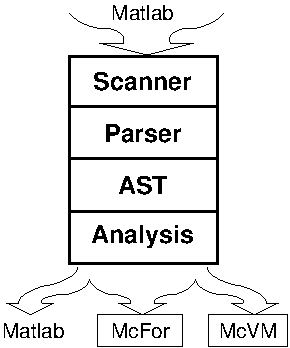
\includegraphics{images/mclab_plain.pdf}}
      \only<2>{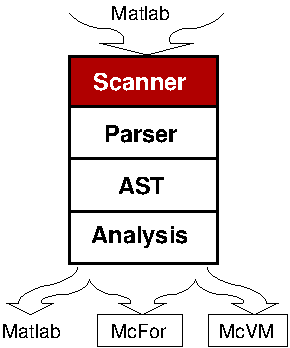
\includegraphics{images/mclab_scanner.pdf}}
      \only<3>{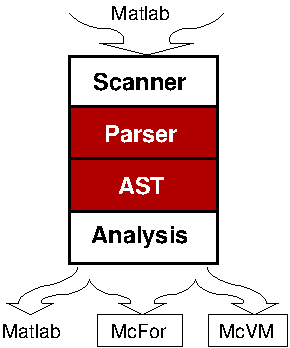
\includegraphics{images/mclab_jastadd.pdf}}
      \only<4>{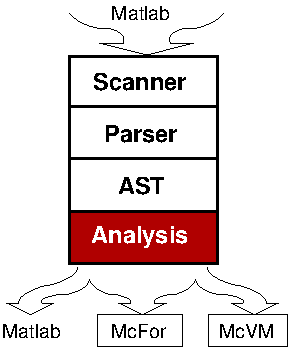
\includegraphics{images/mclab_analysis.pdf}}
    \end{column}
    \begin{column}{5cm}
      \begin{onlyenv}<1>
        \begin{block}{Domain-specific extensions}
          \begin{itemize}
          \item New data structure capabilities
          \item New control flow
          \item Different language constructs
          \end{itemize}
        \end{block}
      \end{onlyenv}
      \begin{onlyenv}<2>
        \begin{block}{Metalexer {\tiny[Casey MSc McGill `09]}
          \vspace{1ex}}
          \begin{center}
            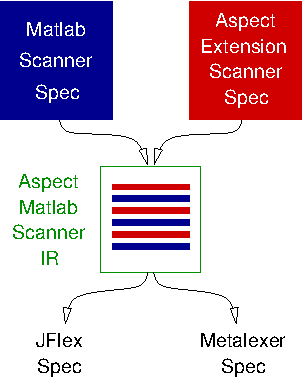
\includegraphics[scale=0.7]{images/metalexer.pdf}
          \end{center}

        \end{block}
      \end{onlyenv}
      \begin{onlyenv}<3>
        \begin{block}{JastAdd {\tiny[Ekman, Hedin SCP `07]}}
          \begin{itemize}
          \item JastAdd parser generator
          \item JastAdd 
            \begin{itemize}
            \item Extensible AST specification
            \item Attribute grammar
            \item Specialized aspect system
            \item Used in abc
            \end{itemize}
          \end{itemize}
        \end{block}
      \end{onlyenv}
      \begin{onlyenv}<4>
        \begin{block}{Analysis framework \\{\tiny[Doherty MSc McGill `10]}}
          \begin{itemize}
          \item Extendable to new language features
          \item Use existing analyses in extensions
          \end{itemize}
        \end{block}
      \end{onlyenv}
    \end{column}
  \end{columns}
\end{frame}
\begin{frame}[t]{Analysis framework}
  \begin{columns}[T]
    \begin{column}{4cm}
      \begin{block}{Base framework}
        \begin{center}
          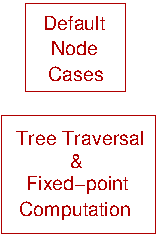
\includegraphics{images/analysis_left.pdf}
        \end{center}
      \end{block}
    \end{column}
    \begin{column}{6cm}
      \begin{onlyenv}<2>
        \begin{block}{A new analysis}
          \begin{center}
            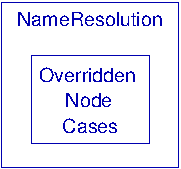
\includegraphics{images/analysis_right.pdf}
          \end{center}
        \end{block}
      \end{onlyenv}
      \begin{onlyenv}<3->
        \begin{block}{Extensions: 
            \only{no new analyses or important nodes}<3>\only{no
              important nodes}<4>\only{new structural
              nodes}<5>\only{changing an analysis}<6>
          }
          \begin{center}
            \begin{onlyenv}<3>
              Handled by class hierarchy and default cases
            \end{onlyenv}
            \begin{onlyenv}<4>
              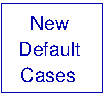
\includegraphics{images/analysis_extension2.pdf}
            \end{onlyenv}
            \begin{onlyenv}<5>
              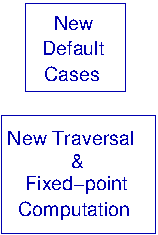
\includegraphics{images/analysis_extension3.pdf}
            \end{onlyenv}
            \begin{onlyenv}<6>
              \includegraphics{images/analysis_extension4.pdf}
            \end{onlyenv}
          \end{center}
        \end{block}
      \end{onlyenv}
    \end{column}
  \end{columns}
  
\end{frame}
